\documentclass[12pt]{article}
%Gumm{\color{blue}i}|065|=)
\usepackage{amsmath, amsfonts, amssymb}
\usepackage[margin=0.5in]{geometry}
\usepackage{xcolor}
\usepackage{graphicx}
\usepackage{amsmath}

\newcommand{\off}[1]{}
\DeclareMathSizes{20}{30}{20}{18}
\usepackage{tikz}


\title{Scratchwork: Schemes}
\date{}
\begin{document}

\sffamily

\maketitle

\noindent 
Let's list some of the examples in Chapter 2 of \textbf{Geometry fo Schemes}
\begin{itemize}
\item $\text{Spec}\;R$ with $R = \mathbb{K}[x,y]/(x^2, xy, y^2, ax+by) \simeq K[t]/(t^2)$ This is a double-point.
\item $\text{Spec}K[x]/(x^3) \not\simeq \text{Spec}K[x,y]/(x^2,xy,y^2)$.  These are examles of triple-points.
\item $X_t = \{ (0,0), (t,0), (0,t) \} \subset \mathbb{A}_K^2$ be three points in the affine plane $\mathbb{A}_K$.  The limit scheme as $t \to 0$ is:
$$ \lim_{t \to 0} X_t = X_0 = \text{Spec}K[x,y]/(x^2, xy, y^2) $$
which is a triple-point. There were three points to begin with and now they are infinitesimally close together. 
\end{itemize}
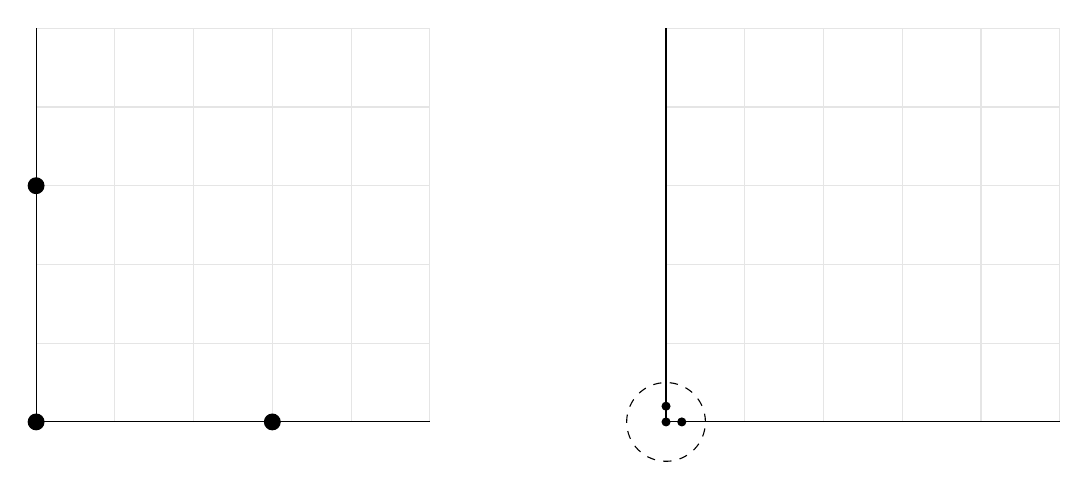
\begin{tikzpicture}
\begin{scope}[xshift=0]

\foreach \a in {0,...,5}{

\draw[black!10!white] (0,\a)--(5,\a);
\draw[black!10!white] (\a,0)--(\a,5);
}

\draw (0,0)--(5,0);
\draw (0,0)--(0,5);
\draw[fill=black] (0,0) circle (0.1);
\draw[fill=black] (0,3) circle (0.1);
\draw[fill=black] (3,0) circle (0.1);



\end{scope}

\begin{scope}[xshift=8cm]

\foreach \a in {0,...,5}{

\draw[black!10!white] (0,\a)--(5,\a);
\draw[black!10!white] (\a,0)--(\a,5);
}

\draw (0,0)--(5,0);
\draw (0,0)--(0,5);
\draw[fill=black] (0,0) circle (0.05);
\draw[fill=black] (0,0.2) circle (0.05);
\draw[fill=black] (0.2,0) circle (0.05);
\draw[dashed] (0,0) circle (0.5);
\end{scope}
\end{tikzpicture} \\
Even more examples:
\begin{itemize}
\item $X = \text{Spec} K[x,y] = (x^2y, xy^2)$ the union of the $x$-axis and the $y$-axis. $\{ x = 0 \} \cup \{ y = 0 \}$.
\end{itemize}
Due to our lack of imagination, these are the minimum we can do.  These arise as limiting situations in classical geometry and we are advised to look at a high-school textbook from here. 
\vfill
\begin{thebibliography}{} 

\item Henri Cohen \textbf{Computational Number Theory in Relation with L-Functions} \texttt{arXiv:1809.10904}

\item Hugh Montgomery, Robert Vaughan \textbf{Multiplicative Number Theory I: Classical Theory} \\ (Cambridge Studies in Advanced Mathematics, \#97) Cambridge University Press, 2010.

\item Yitzhak Katznelson \textbf{An Introduction to Harmonic Analysis} (Cambridge Mathematical Library) \\ Cambridge University Press, 2004.

\end{thebibliography}

\begin{thebibliography}{} 

\item David Eisenbud, Joe Harris.  \textbf{The Geometry of Schemes}. (GTM \#197) Springer, 2000.
\item Ravi Vakil \textbf{Foundations of Algebraic Geometry} (online) \texttt{http://math.stanford.edu/~vakil/216blog/}

\end{thebibliography}


\end{document}